
\section{Placement}
\end{multicols}
{
    \centering
    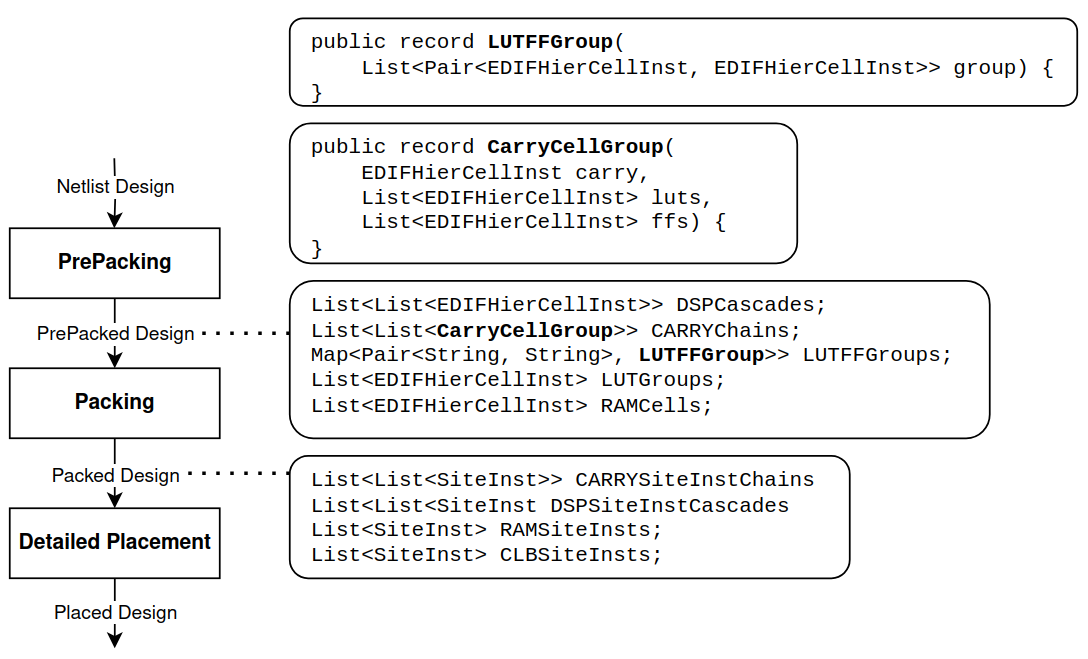
\includegraphics[width=0.8\columnwidth]{figures/substages.png}
    \captionof{figure}{The data classes populated at each substage: \texttt{PrepackedDesign}, \texttt{PackedDesign}, and \texttt{PlacedDesign}.}
    \label{fig:substages}
}
\begin{multicols}{2}
\label{sec:simulated_annealing}
With a basic understanding of FPGA architecture, design placement, and RapidWright, we have all the necessary pieces to implement our SA placer. 
Here we outline in detail each substage of our implementation: PrePacking, Packing, and Placement. 
Shown in Figure \ref{fig:edif_design_device} is an overview of the placement workflow. 
Figure \ref{fig:substages} shows the data structures of RapidWright objects that are populated at each stage: \texttt{PrepackedDesign}, which is a group of data structures around \texttt{EDIFHierCellInst}s, \texttt{PackedDesign}, which is a group fo data structures around \texttt{SiteInst}s, and finally, \texttt{PlacedDesign}, which is simply captured by the final RapidWright \texttt{Design} object. 

\vspace{0.5cm}
{
    \centering
    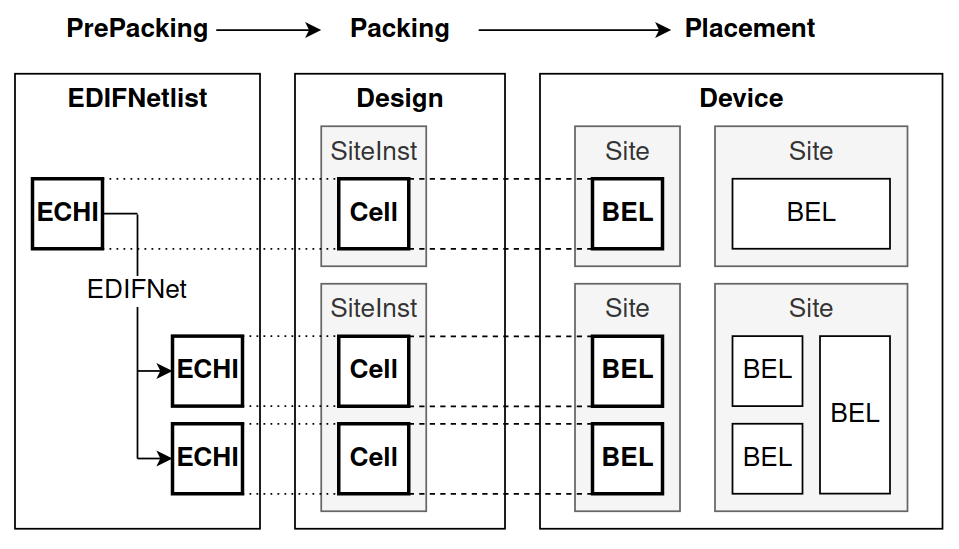
\includegraphics[width=0.9\columnwidth]{figures/edif_design_device.png}
    \captionof{figure}{Our placement workflow}
    \label{fig:edif_design_device}
}


\subsection{Prepacking}
\label{subsec:prepacking}


The first step in our placement flow is \textbf{prepacking}. 
Recall from the 7-Series architecture that there are certain multi-cell structures that must adhere to certain placements constraints to ensure legality, and by design, to minimize wirelength. 
The job of the prepacker is to traverse the raw EDIF netlist, detect these multi-cell structures, and consolidate these cells into clusters or groups of clusters that naturally reflect these placement constraints. 

Recall that \texttt{CARRY4} chains must necessarily be placed vertically and consecutively across a column of SLICEs in ascending order. 
Likewise, \texttt{DSP48E1} cascades must necessarily be placed vertically and consecutively across a column of \texttt{DSP48E1} Sites in ascending order. 
A LUT-FF pair may be placed freely, but should be placed in the same lane within the same SLICE to minimize wirelength.

The raw EDIF netlist only tells us the list of nets and the cell ports that they connect to. 
It does not report the presence of any multi-cell structures (\texttt{CARRY4} chains, etc.). 
Thus, we must traverse the netlist to detect these multi-cell structures and store that structure information in a class we will call \texttt{PrepackedDesign}.

The code snippet in \ref{lst:carry_chains} shows how one can detect and collect these \texttt{CARRY4} chains using RapidWright. 
We first collect the cells in the design that are of type \texttt{CARRY4}, then iteratively traverse their Carry-Out (\texttt{CO}) to Carry-In (\texttt{CI}) nets to find incident \texttt{CARRY4} cells.
Each \texttt{CARRY4} chain has an anchor cell and a tail cell where the chain terminates.
The anchor is found when the \texttt{CI} net connects to Ground (\texttt{GND}), while the tail is found when the \texttt{CO} port is null. 
We can further detect if there are \texttt{LUT}s or \texttt{FF}s connected to the \texttt{CARRY4} cell and store that information in a data structure we will call \texttt{CarryCellGroup} as defined in figure \ref{fig:substages}.
This will help us in knowing which cells can be packed together into the same \texttt{Site} in the subsequent stages. 

Similarly, \texttt{DSP48E1} cascades can be found and collected by traversing the \texttt{PCOUT} \texttt{ACOUT} and \texttt{BCOUT} nets.
\texttt{LUT-FF} pairs can be found by inspecting the LUT output (O) net and checking for FF input (DI) ports. 
We can bucket these LUT-FF pairs by finding the set of unique \texttt{CE} \texttt{SR} net pairs to know which group of LUT-FF pairs can be placed within the same \texttt{Site}. 

We detect the presence of these multi-cellular structures and consolidate that information into our \texttt{PrepackedDesign} object in preparation for the following Packing stage. 


\end{multicols}
{
    \centering
    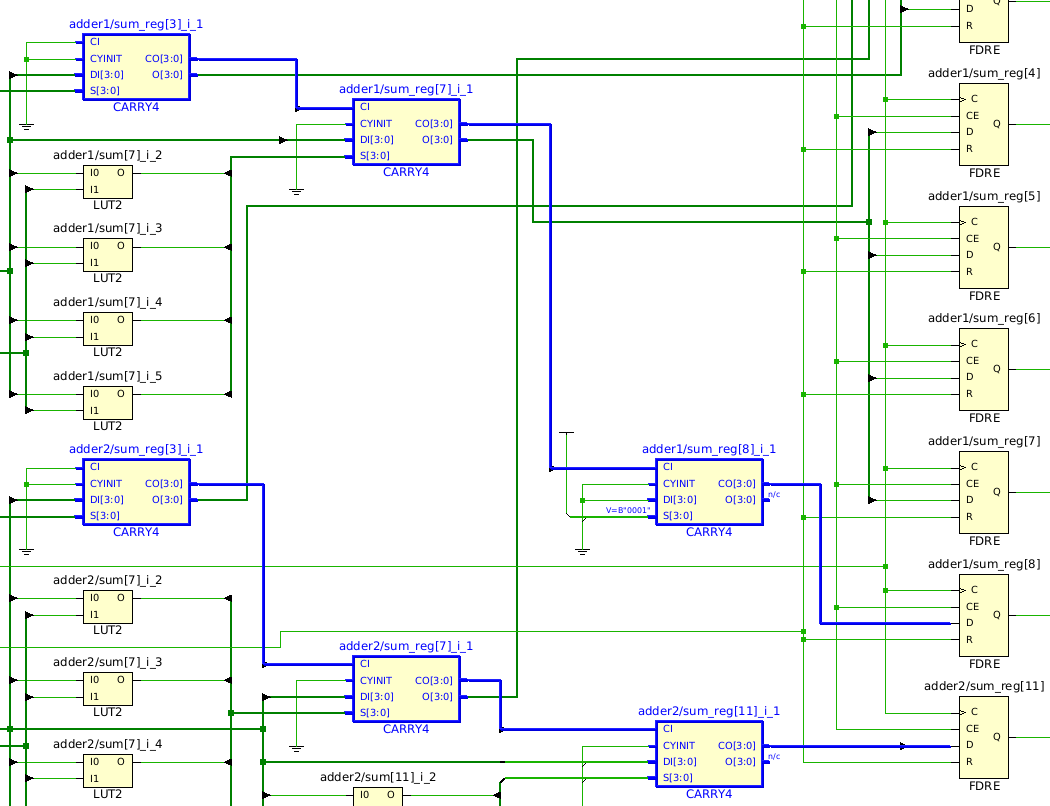
\includegraphics[width=0.8\columnwidth]{figures/carry_chain_traversal.png}
    \captionof{figure}{A netlist with two \texttt{CARRY4} chains, each of size 3}
    \label{fig:carry_chain_traversal}
}
\begin{multicols}{2}


\begin{lstlisting}[caption={Code Printout}]
Anchor Cell: adder2/sum_reg[3]_i_1, CellType: CARRY4
	Cell: adder2/sum_reg[7]_i_1, CellType: CARRY4
	Cell: adder2/sum_reg[11]_i_1, CellType: CARRY4
Anchor Cell: adder1/sum_reg[3]_i_1, CellType: CARRY4
	Cell: adder1/sum_reg[7]_i_1, CellType: CARRY4
	Cell: adder1/sum_reg[8]_i_1, CellType: CARRY4
\end{lstlisting}


\begin{lstlisting}[language=java, caption={Finding and storing carry chains.}, label={lst:carry_chains}]
Design design = Design.readCheckpoint("synth.dcp")
EDIFNetlist netlist = design.getNetlist();
List<EDIFCellInst> ecis = netlist.getAllLeafCellInstances();

// Select only the carry cells.
List<EDIFCellInst> carryCells = new ArrayList<>();
for (EDIFCellInst eci : ecis) {
    if (eci.getCellName().equals("CARRY4"))
        carryCells.add(eci);
}

// Find and remove carry chains until the list is empty
List<List<EDIFCellInst>> carryChains = new ArrayList<>();
while (!carryCells.isEmpty()) {
    // Arbitrarily set "currentCell" pointer to a cell in the list
    EDIFCellInst currentCell = carryCells.get(0);

    // Find this carry chain anchor.
    // Traverse the Carry-In (CI) to Carry-Out (CO) nets.
    // Anchor is found when net on the CI Port is Ground.
    while (true) {
        System.out.println(currentCell);
        // Access the CI port on this cell.
        EDIFPortInst sinkPort = currentCell.getPortInst("CI");
        // Access the net on this CI port.
        EDIFNet net = sinkPort.getNet();
        if (net.isGND()) {
            // Found this chain anchor!
            break;
        }
        // Get all ports on this net.
        List<EDIFPortInst> netPorts = net.getPortInsts();
        for (EDIFPortInst netPort : netPorts) {
            // Access the port belonging to another carry cell.
            EDIFCellInst sourceCell = netPort.getCellInst();
            if (sourceCell.getCellName().equals("CARRY4")) {
                // Move the "currentCell" pointer
                currentCell = sourceCell;
                break;
            }
        }
    }



    // Now we have the chain anchor as currentCell.
    // Now traverse in the opposite direction to find the chain tail.
    // Tail is found when the CO Port is null.
    // Collect the chain cells into an ordred list.
    List<EDIFCellInst> currentChain = new ArrayList<>();
    currentChain.add(currentCell);
    while (true) {
        EDIFPortInst sourcePort = currentCell.getPortInst("CO[3]");
        if (sourcePort == null) {
            // Found this chain's tail!
            break;
        }
        EDIFNet net = sourcePort.getNet();
        List<EDIFPortInst> netPorts = net.getPortInsts();
        for (EDIFPortInst netPort : netPorts) {
            EDIFCellInst sinkCell = netPort.getCellInst();
            if (netPort.getName().equals("CI") &&
                    sinkCell.getCellName().equals("CARRY4")) {
                currentCell = sinkCell;
                // Add the cell to the chain list.
                currentChain.add(currentCell);
                break;
            }
        }
    }
    // Add currentChain to the list of chains
    carryChains.add(currentChain);
    // Remove currentChain from the list of cells
    carryCells.removeAll(currentChain);
} // end while()

// Print out the carry chains. 
for (List<EDIFCellInst> chain : chains) {
    for (int i = 0; i < chain.size(); i++) {
        EDIFCellInst carry = chain.get(i);
        if (i == 0) {
            writer.write("\nAnchor Cell: " + carry.getName() + 
                ", CellType: " + carry.getCellName());
        } else {
            writer.write("\n\tCell: " + carry.getName() + 
                ", CellType: " + carry.getCellName());
        }
    }
}
\end{lstlisting}
\newpage




\subsection{Packing}
\label{subsec:packing}
Now that we have our \texttt{PrepackedDesign} object keeping track of multi-cell structures on the \texttt{edif} level, we can start packing them into \texttt{SiteInst} objects on the \texttt{design} level. 
Below are some of the most relevant classes from the \texttt{design} package for this task.
\begin{itemize}
    \item \texttt{Cell}: A cell corresponds to the leaf cell within the logical netlist \texttt{EDIFCellInst} and provides a mapping to a physical location BEL on the device. A cell can be created directly out of an \texttt{EDIFCellInst} to inherit all of its \texttt{edif} properties on the \texttt{design} level.
    \item \texttt{Net}: Represents the physical net to be routed (both inter-site and intra-site). When an \texttt{Cell} is created out of an \texttt{EDIFCellInst}, the \texttt{Net}s are automatically created out of its corresponding \texttt{EDIFNet}s.
    \item \texttt{SiteInst}: An instance of a \texttt{Site} on the \texttt{Device}. Carries the mapping information between the \texttt{BEL}s in a \texttt{Site} and the \texttt{Cell}s assigned to them. Also keeps track of the intra-Site routing information within (\texttt{Net}s, \texttt{SitePinInst}s, \texttt{SitePIP}s, etc.).
    \item \texttt{SitePIP}: A Programmable Interconnect Point (PIP) in a \texttt{Site}. Represents the fuses in intra-Site routing \texttt{BEL}s. 
    \item \texttt{SitePinInst}: An instance of a \texttt{SitePin} on a \texttt{Site}. These objects serve as the interface between intra-Site routing and general inter-Site routing. 
\end{itemize}
\columnbreak


A new \texttt{SiteInst} is created by populating its BELs with existing \texttt{EDIFHierCellInst} objects from the \texttt{EDIFNetlist}, and is immediately placed on a specific \texttt{Site}. 
The packer therefore assigns an initial placement to every \texttt{SiteInst} before the simulated‐annealing stage randomizes their positions. 
During this packing phase, we simply pseudorandomly map \texttt{design} \texttt{SiteInst}s onto \texttt{device} \texttt{Site}s in coordinate order as they are generated (e.g., the first \texttt{SiteInst} onto \texttt{SLICEL\_X0Y0}, the second onto \texttt{SLICEL\_X0Y1}, and so on). 

One can think of a \texttt{design} \texttt{SiteInst} as a movable square peg and the corresponding \texttt{device} \texttt{Site} as a fixed square hole. 
Both \texttt{SiteInst}s and \texttt{Site}s come in various shapes or types (\texttt{SLICEL}, \texttt{SLICEM}, \texttt{DSP48E1}, etc.) and placement is only allowed between compatible pairs. 
For example, a \texttt{RAMB48E1} \texttt{SiteInst} can only be placed on a \texttt{RAMB48E1} \texttt{Site}.
A \texttt{DSP48E1} \texttt{SiteInst} can only be placed on a \texttt{DSP48E1} \texttt{Site}.
A \texttt{SLICEL} \texttt{SiteInst} may occupy either a \texttt{SLICEL} or a \texttt{SLICEM} \texttt{Site}, whereas a \texttt{SLICEM} \texttt{SiteInst} can only be placed on a \texttt{SLICEM} \texttt{Site}.
These constraints must be followed as the \texttt{SiteInst}s move across the device throughout the placement stage to ensure legality. 


\end{multicols}
\begin{lstlisting}[caption=\texttt{SiteInst} constructor and methods.]
SiteInst Constructor: 
    SiteInst(String name, Design design, SiteTypeEnum type, Site site)

Most relevant SiteInst Methods:
    createCell(EDIFHierCellInst inst, BEL bel) // Populating the SiteInst BELs with Cells
    unplace() // Unplacing the SiteInst from its current Site
    place(Site site) // Placing an unplaced SiteInst onto a Site
    routeSite() // Attempt to automatically route all intra-Site nets (manual intervention likely required)
    routeIntraSiteNet(Net net, BELPin src, BELPin snk) // Manually route an intra-Site net

Example:
    SiteInst si = new SiteInst("mySiteInst", design, SiteTypeEnum.SLICEL, device.getSite("SLICEL_X0Y1"));
    si.createCell(someFDRECell, si.getBEL("AFF"));
    si.routeSite();
    si.unplace();
    si.place(device.getSite("SLICEL_X15Y33"));
    // In Simulated Annealing, SiteInst objects will be unplaced() and placed() many times to converge to an optimal solution. 
    // All Cell-BEL mapping and intra-Site routing is preserved when a SiteInst is moved. 

\end{lstlisting}


\begin{lstlisting}[language=java, caption={Packing an individual \texttt{CarryCellGroup} into one \texttt{SLICEL} \texttt{SiteInst}s.}, label={lst:single_carry_chains}]
protected String[] FF_BELS = new String[] { "AFF", "BFF", "CFF", "DFF" };
protected String[] LUT6_BELS = new String[] { "A6LUT", "B6LUT", "C6LUT", "D6LUT" };

private void packCarrySite(CarryCellGroup carryCellGroup, SiteInst si) {
    // potential bug: what guarantees that all of the FFs connected to the CARRY4 all share the same CE and Reset?
    for (int i = 0; i < 4; i++) {
        EDIFHierCellInst ff = carryCellGroup.ffs().get(i);
        if (ff != null)
            si.createCell(ff, si.getBEL(FF_BELS[i]));
        EDIFHierCellInst lut = carryCellGroup.luts().get(i);
        if (lut != null)
            si.createCell(lut, si.getBEL(LUT6_BELS[i]));
        // carry site LUTs MUST be placed on LUT6 BELs.
        // only LUT6/O6 can connect to CARRY4/S0
    }
    si.createCell(carryCellGroup.carry(), si.getBEL("CARRY4"));
    // default intrasite routing
    si.routeSite();
    // sometimes the default routeSite() is insufficient, so some manual
    // intervention is required
    rerouteCarryNets(si);
    rerouteFFClkSrCeNets(si);
} // end placeCarrySite()
\end{lstlisting}

\newpage
\begin{lstlisting}[language=java, caption={Packing \texttt{CarryCellGroup}s into \texttt{SLICEL} \texttt{SiteInst}s.}, label={lst:carry_chains}]
private List<List<SiteInst>> packCarryChains(List<List<CarryCellGroup>> EDIFCarryChains)
        throws IOException {
    List<List<SiteInst>> siteInstChains = new ArrayList<>();
    writer.write("\n\nPacking carry chains... (" + EDIFCarryChains.size() + ")");
    for (List<CarryCellGroup> edifChain : EDIFCarryChains) {
        List<SiteInst> siteInstChain = new ArrayList<>();
        writer.write("\n\t\tChain Size: (" + edifChain.size() + "), Chain Anchor: "
                + edifChain.get(0).carry().getFullHierarchicalInstName());
        Site anchorSite = selectCarryAnchorSite(edifChain.size());
        SiteTypeEnum selectedSiteType = anchorSite.getSiteTypeEnum();
        for (int i = 0; i < edifChain.size(); i++) {
            Site site = (i == 0) ? anchorSite
                    : device.getSite("SLICE_X" + anchorSite.getInstanceX() + "Y" + (anchorSite.getInstanceY() + i));
            SiteInst si = new SiteInst(edifChain.get(i).carry().getFullHierarchicalInstName(), design,
                    selectedSiteType,
                    site);
            packCarrySite(edifChain.get(i), si);
            if (i == 0) { // additional routing logic for anchor site
                Net CINNet = si.getNetFromSiteWire("CIN");
                CINNet.removePin(si.getSitePinInst("CIN"));
                si.addSitePIP(si.getSitePIP("PRECYINIT", "0"));
            }
            occupiedSites.get(selectedSiteType).add(site);
            availableSites.get(selectedSiteType).remove(site);
            siteInstChain.add(si);
        }
        siteInstChains.add(siteInstChain);
    } // end for (List<EDIFCellInst> chain : EDIFCarryChains)
    return siteInstChains;
} // end packCarryChains()

\end{lstlisting}


\begin{lstlisting}[language=java, caption={Manually rerouting intra-Site nets in a \texttt{SLICEL} containing \texttt{CARRY4}}]
    protected String[] FF_BELS = new String[] { "AFF", "BFF", "CFF", "DFF" };
    private void rerouteCarryNets(SiteInst si) {
        // activate PIPs for CARRY4/COUT
        si.addSitePIP(si.getSitePIP("COUTUSED", "0"));
        // undo default CARRY4/DI nets
        SitePinInst AX = si.getSitePinInst("AX");
        if (AX != null)
            si.unrouteIntraSiteNet(AX.getBELPin(), si.getBELPin("ACY0", "AX"));
        SitePinInst DX = si.getSitePinInst("DX");
        if (DX != null)
            si.unrouteIntraSiteNet(DX.getBELPin(), si.getBELPin("DCY0", "DX"));
        // activate PIPs for CARRY4/DI pins
        si.addSitePIP(si.getSitePIP("DCY0", "DX"));
        si.addSitePIP(si.getSitePIP("CCY0", "CX"));
        si.addSitePIP(si.getSitePIP("BCY0", "BX"));
        si.addSitePIP(si.getSitePIP("ACY0", "AX"));
        // remove stray CARRY4/CO nets
        if (si.getNetFromSiteWire("CARRY4_CO2") != null)
            design.removeNet(si.getNetFromSiteWire("CARRY4_CO2"));
        if (si.getNetFromSiteWire("CARRY4_CO1") != null)
            design.removeNet(si.getNetFromSiteWire("CARRY4_CO1"));
        if (si.getNetFromSiteWire("CARRY4_CO0") != null)
            design.removeNet(si.getNetFromSiteWire("CARRY4_CO0"));
        // add default XOR PIPs for unused FFs
        for (String FF : FF_BELS)
            if (si.getCell(FF) == null)
                si.addSitePIP(si.getSitePIP(FF.charAt(0) + "OUTMUX", "XOR"));
    } // end rerouteCarryNets()
\end{lstlisting}
\begin{multicols}{2}



\subsection{Placement}
    \label{subsec:placement}
    Up until now we have only organized the logical \texttt{EDIFHierCellInst}s into \texttt{SiteInst}s. 
    This is where simulated annealing actually begins where we actually place the \texttt{SiteInst}s onto physical \texttt{Site}s on the \texttt{device} level. 

